\chapter{Testování}
\label{ch:testovani}

\section{Zdrojové snímky}
Důležitým základem pro otestování algoritmu pro automatickou detekci příznaků onemocnění VPMD je mít dostatečně velké množství snímků sítnic. Tyto snímky by měly tvořit reprezentativní soubor zahrnující charakteristické příznaky tohoto onemocnění.

V~průběhu tvorby této práce byly využity databáze ADCIS \cite{db_adcis}, FIRE \cite{db_fire}, HRF \cite{db_hrf}, diaretdb0 \cite{db_diaret0} a diaretdb1 \cite{db_diaret1}. Databáze ADCIS je složena z~56 barevných digitálních snímků ve formátu JPG v~rozlišení 2544$\times$1696~pixelů a 1440$\times$960~pixelů. Z~těchto 56 snímků se na 37 vyskytují exudáty a zbylých 19 snímků zachycuje zdravé sítnice. Databáze FIRE obsahuje 42 snímků ve formátu JPG v~rozlišení 2912$\times$2912~pixelů. Tyto snímky taktéž zahrnují zdravé sítnice a sítnice s~těžkými exudáty. Databáze HRF je rozdělena na zdravé sítnice a sítnice obsahující příznaky diabetické retinopatie. Obě tyto skupiny obsahují 15 snímků s~rozlišením 3504$\times$2336~pixelů ve formátu JPG. Databáze diaretdb0 a diaretdb1 dohromady zahrnují 219 barevných digitálních snímků ve formátu PNG s~rozlišením 1500$\times$1152~pixelů obsahující nálezy jako neovaskularizaci, hemoragie a v~neposlední řadě také exudáty a drúzy. Další použitý soubor snímků byl pořízen na Fakultě informačních technologií v~Brně, která je vybavena vlastní fundus kamerou. Tento soubor obsahuje celkem 60 fotek sítnic, které byly pořízeny studenty. Tyto fotky neobsahují žádné příznaky VPMD. 

Dohromady je k~dispozici 407 snímků získaných pomocí fundus kamery. Souhrn informací o~těchto databázích je uveden v~tabulce \ref{tab:databases}.

Databáze ADCIS a FIRE obsahovaly velké množství obrázků zachycujících stejné sítnice, mezi kterými byly minimální rozdíly. Aby tyto podobné a opakující se obrázky nezkreslovaly výsledky testovaní, rozhodl jsem se pro jejich vyloučení.

\begin{table}[ht]
  \begin{center}	
    \begin{tabular}{|c|c|c|c|}
      \hline
      \textbf{Databáze} & \textbf{Rozlišení} & \textbf{Formát} & \textbf{Počet snímků} \\
      \hline
      ADCIS     & \makecell{2544$\times$1696\\ 1440$\times$960} & JPG &  56\\
      \hline
      FIRE      & 2912$\times$2912                            & JPG &  42\\
      \hline
      HRF       & 3504$\times$2336                            & JPG &  30\\
      \hline
      diaretdb0 & 1500$\times$1152                            & PNG & 130\\
      \hline
      diaretdb1 & 1500$\times$1152                            & PNG &  89\\
      \hline
      FIT       & 3888$\times$2592                            & JPG &  60\\
      \hline
      \multicolumn{3}{|r|}{$\sum$}                                   & 407\\
      \hline
    \end{tabular}
  \caption{Použité databáze.}
  \label{tab:databases}
  \end{center}
\end{table}


\section{Testování detekce optického disku a fovey}
Pro účely testování byla implementována samostatná třída \emph{Tester} poskytující metody pro sběr dat a jejich následné vyhodnocení. Tato třída využívá knihovny \emph{filesystem} pro rekurzivní procházení adresářové struktury obsahující snímky daných databází.

\subsection*{Sběr dat} 
V~prvním kroku je potřeba vytvořit referenční soubor dat, se kterým se budou porovnávat výsledky mého algoritmu. Člověk nemusí mít odborné znalosti očního lékaře pro lokalizaci optického disku a fovey na sítnici lidského oka a pouze stačí, pokud je informovaným laikem zasvěceným do této problematiky. Díky tomu jsem sběr dat pro testování detekce optického disku a fovey mohl provést sám bez nutnosti asistence oftalmologa. 

Testovací třída obsahuje metodu pro určení pozic těchto očních struktur uživatelem. Jako vstupní parametr této metody je předána cesta k~adresáři obsahující snímky určené k~testování. Všechny tyto snímky se postupně prochází a zobrazují se na obrazovce, kde uživatel prvním kliknutím levého tlačítka myši do obrázku určí střed optického disku a druhým kliknutím určí střed fovey. Získané polohy se ukládají do souboru \emph{groundtruth} umístěného v~adresáři dané databáze. Každý snímek má svůj záznam nacházející se na samostatném řádku, kde jsou středníkem odděleny jednotlivé informace. Nejprve se ukládá relativní cesta k~danému snímku vzhledem k~umístění tohoto souboru, následně jsou zaznamenány souřadnice optického disku a jako poslední jsou uloženy souřadnice fovey. Po druhém kliknutí myši a uložením daného záznamu se automaticky načte další obrázek. Takhle to probíhá do doby, než jsou zpracovány všechny snímky v~daném adresáři.

\subsection*{Vyhodnocení dat}
Další z~metod třídy \emph{Tester} realizuje samotné testování. Jako vstupní parametr je předána cesta ke \emph{groundtruth} souboru, který byl vytvořen v~předchozím kroku. Do jeho adresáře se vytvoří soubor \emph{test\_results} obsahující výsledky tohoto testování. 

Ze vstupního souboru se parsují jednotlivé záznamy, ze kterých se načtou konkrétní snímky. Každý tento snímek je předzpracován a následně je nad ním spuštěn algoritmus pro detekci optického disku. Získaná data se porovnávají s~daty obsaženými v~aktuálním záznamu. Porovnání je založeno na základě vzdálenosti ručně určeného středu se středem, který vypočítal algoritmus. 

Vzdálenost $|AB|$ dvou bodů $A[x_A, y_A]$ a $B[x_B, y_B]$ v~rovině je dána vzorcem:

\begin{equation}
  |AB| = \sqrt{(x_B - x_A)^2 + (y_B - y_A)^2}
\end{equation}

Pokud je vzdálenost mezi referenčním středem uvedeným v~záznamu a nalezeným středem optického disku menší než $2/3$ jeho poloměru, byl úspěšně detekován. Pokud je tato vzdálenost větší nebo rovna $2/3$ poloměru optického disku, detekce fovey se už netestuje, protože algoritmus pro její lokalizaci je závislý na umístění právě optického disku. Naopak v~případě jeho úspěšné lokalizace se detekce fovey spustí a následně se porovnává získaný střed s~referenčním středem, kde ke správné detekci došlo pouze v~případě, kdy jsou tyto středy od sebe vzdáleny maximálně do velikosti poloměru fovey.

Na konci souboru s~výsledky testování dané databáze je uvedena statistika. Z~ní lze vyčíst, na kolika snímcích byl úspěšně detekován optický disk z~jejich celkového počtu, na kolika fovea a jaká je celková úspěšnost jednotlivých algoritmů. Vzhledem k~tomu, že je detekce fovey závislá na lokalizaci optického disku, je zde uvedena i její úspěšnost vzhledem k~počtu správně nalezených optických disků.

\subsection*{Výsledky}
Výsledky detekce optického disku jsou shrnuty v~tabulce \ref{tab:results_od}. Většina nesprávných detekcí se nacházela na snímcích, které byly buď velmi špatně osvětleny, nebo obsahovaly optický disk, který splýval s~pozadím sítnice. 

Výsledky detekce fovey jsou shrnuty v~tabulce \ref{tab:results_fovea}, která obsahuje úspěšnost detekce vzhledem k~celkovému počtu snímků a také úspěšnost vzhledem k~celkovému počtu úspěšně detekovaných optických disků. Pokud se podaří správně lokalizovat optický disk, fovea je následně téměř vždy úspěšně nalezena. Po prozkoumání nesprávných detekcí z~výsledků vyplývá, že úspěšnost algoritmu je přímo úměrná kvalitě testovaných snímků. 

\begin{table}[ht]
  \begin{center}	
    \begin{tabular}{|c|c|c|}
      \hline
      \textbf{Databáze} & \textbf{Detekce} & \textbf{Úspěšnost}\\
      \hline
      ADCIS     & $53/56$   & 94,64 \% \\
      \hline
      FIRE      & $42/42$   & 100 \% \\
      \hline
      HRF       & $27/30$   & 90,00 \% \\
      \hline
      diaretdb0 & $119/130$ & 91,54 \% \\
      \hline
      diaretdb1 & $79/89$   & 88,76 \% \\
      \hline
      FIT       & $54/60$   & 90,00 \% \\
      \hline
      \hline
      \textbf{Celkem} & \textbf{374/407} & \textbf{91,89 \%} \\
      \hline
    \end{tabular}
  \caption{Výsledky testování detekce optického disku.}
  \label{tab:results_od}
  \end{center}
\end{table}

\begin{table}[ht]
  \begin{center}	
    \begin{tabular}{|c|c|c|c|c|}
      \hline
      \textbf{Databáze} & \textbf{Detekce} & \textbf{Úspěšnost} & \textbf{Detekce po úpravě} & \textbf{Výsledná úspěšnost}\\
      \hline
      ADCIS     & $51/56$   & 91,07 \% & $51/53$   & 96,23 \%\\
      \hline
      FIRE      & $41/42$   & 97,62 \% & $41/42$   & 97,62 \%\\
      \hline
      HRF       & $27/30$   & 90,00 \% & $27/27$   & 100 \%\\
      \hline
      diaretdb0 & $114/130$ & 87,69 \% & $114/119$ & 92,44 \%\\
      \hline
      diaretdb1 & $76/89$   & 85,39 \% & $76/79$   & 96,20 \%\\
      \hline
      FIT       & $54/60$   & 90,00 \% & $54/54$   & 100 \%\\
      \hline
      \hline
      \textbf{Celkem} & \textbf{363/407} & \textbf{89,19 \%} & \textbf{363/374} & \textbf{97.06 \%} \\
      \hline
    \end{tabular}
  \caption{Výsledky testování detekce fovey.}
  \label{tab:results_fovea}
  \end{center}
\end{table}


\section{Testování detekce drúz a exudátů}
Vyhodnocení úspěšnosti detekce nálezů jsem již nemohl provést sám, protože se poměrně těžce identifikují, proto je zapotřebí mít zkušenosti a odborné znalosti očního lékaře. Z~tohoto důvodu jsem si domluvil schůzku s~doktorem Tomášem Mňukem, který působí ve Fakultní nemocnici u~sv. Anny v~Brně a který mi velmi pomohl při klasifikaci těchto nálezů.

Testovací program postupně zobrazoval dva obrázky, kde první představoval výchozí nezměněný snímek a na druhém byly vyznačeny příznaky onemocnění detekované mým algoritmem. To lze vidět na obrázku \ref{pic:chap06_test_process}.

\begin{figure}[h]
  \begin{center}
    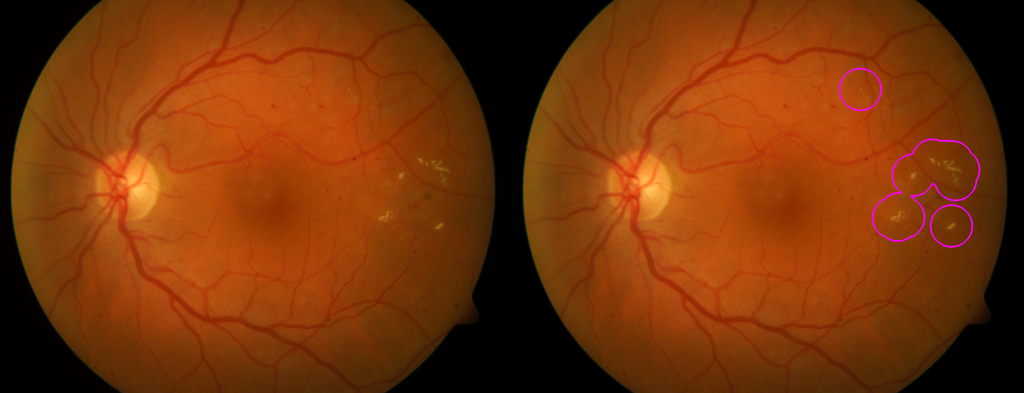
\includegraphics[width=\linewidth]{chap06_test_process}
    \caption{Testovací proces.}
    \label{pic:chap06_test_process}
  \end{center}
\end{figure}

Samotné vyhodnocování probíhalo manuálně, kde tyto snímky byly posouzeny doktorem. Ve vymezeném čase, který jsme spolu strávili, jsme však stihli otestovat pouze 50 snímků a to prvních 30 z~databáze diaretdb0 a prvních 20 z~databáze diaretdb1. Na snímcích se posuzovalo, zdali algoritmus správně detekoval drúzy a exudáty a zdali je detekoval všechny. Z~celkového počtu 50 snímků byly správně detekovány všechny drúzy či exudáty na 25, na 22 snímcích byla detekována většina, ale některé chyběly a na 3 snímcích byly kromě správných nálezů detekovány i oblasti, které nálezy nepředstavují. Hlavní příčinou nesprávné identifikace nálezů byla chyba při detekci krevního řečiště či optického disku. V~žádném z~případů se však nestalo, že by sítnice trpěla onemocněním VPMD nebo diabetické retinopatie a algoritmus by žádný z~příznaků nenalezl.

Já sám jsem již bez odborného dozoru provedl testování nad databázemi ADCIS a HRF, které jsou podle svého zdroje rozděleny na zdravé sítnice a sítnice s~nálezy, a souborem snímků sítnic pořízených na Fakultě informačních technologií v~Brně, u~kterého předpokládám, že obsahuje zdravé sítnice studentů. Dohromady bylo testováno 94 snímků, kde z~tohoto počtu byly na 21 snímcích nalezeny nějaké nálezy. Ty byly detekovány špatně a to hlavně z~důvodu, že se jednalo buď o~odlesky vzniklé špatným focením, nebo o~odlesky na sítnici, které se vyskytují u~mladých lidí. Podle pana doktora by však nemělo nastat, že by člověk trpěl VPMD a zároveň by měl na své sítnici tyto odlesky. Pokud by se tedy algoritmus použil pouze u~starších lidí, nemělo by k~těmto špatným detekcím docházet.
